\subsection{Navier-Stokes Physics Informed Neural Network solver to simulate two-dimensional cylinder wake flow}

I implemented a physics informed neural network that can train on limited simulation data and approximate the physical evolution of fluid flow described by the NS equations. My PINN model is based on the same principles as the one described in Raissi et al.\cite{Raissi2019}, where the NS equations are encoded into the equations loss term. If we consider the non-dimensional NS equations below:
\begin{align}
    u_{t} + (uu_{x} = vu_{y}) &= -p_{x} + \frac{1}{Re} (u_{xx} + u_{yy}) \\
    v_{t} + (uv_{x} = vv_{y}) &= -p_{y} + \frac{1}{Re} (v_{xx} + v_{yy})
\end{align} 

\noindent where $Re$ is the Reynolds number, we can formulate two equation loss functions for the PINN.
\begin{align}
    f &:= u_{t} + (uu_{x} = vu_{y}) + p_{x} - \frac{1}{Re} (u_{xx} + u_{yy}) \\
    g &:= v_{t} + (uv_{x} = vv_{y}) +p_{y} - \frac{1}{Re} (v_{xx} + v_{yy})
\end{align} 

\noindent Combining these equation loss functions with the data loss results in the following mean-squared error term:
\begin{align}
    MSE := \frac{1}{N} \Sigma^{N}_{i = 1} (|u(t^{i}, x^{i}, y^{i}) - u^{i}|^2 +  |v(t^{i}, x^{i}, y^{i}) - v^{i}|^2) + \frac{1}{N} \Sigma^{N}_{i = 1} (|f(t^{i}, x^{i}, y^{i})|^2 + |g(t^{i}, x^{i}, y^{i})|^2)
\end{align}

\noindent The first term in equation (11) minimizes data loss from the model approximation, while the second term minimizes equation loss, since $f$ and $g$ are supposed to be zero according to the NS equations.\\

I implemented the PINN using the NumPy and Tensorflow2 libraries in python. Implementation with the Tensorflow2 library makes the model significantly more readable and modular. Additionally,  I structured the model code following object-oriented design principles to make the model more user friendly.

\subsubsection{PINN Training and Testing Data}
For this initial PINN model implementation, I decided to use the high quality cylinder wake-flow simulation data from Raissi et al. \cite{Raissi2019}, which was acquired by evolving the domain described in Figure \ref{fig:Pinn Domain}. I have assumed a uniform free stream velocity profile imposed at the left boundary, a zero pressure outflow condition imposed at the right boundary located 25 diameters downstream of the cylinder, and periodicity for the top and bottom boundaries of the $[15, 25] \times [8, 8]$ domain. The free stream velocity is $u_{\infty} = 1$, the cylinder diameter is $D = 1$, and the Reynold's number is set to $Re = 100$. The training and testing data subdomain has been identified in with the black rectangle in the figure below. Additionally, the training data arrays are also visualized in Figure \ref{fig:Pinn Domain}, where the scattered points in the arrays representing the streamwise ($u$) and transverse ($v$) velocity components indicate the $N = 5000$ training data (less than $1 \%$ of available data). Testing data are selected as select slices from the $u$ and $v$ arrays (the colorful slices in Figure \ref{fig:Pinn Domain} bottom)

\begin{figure}[h]
    \centering
    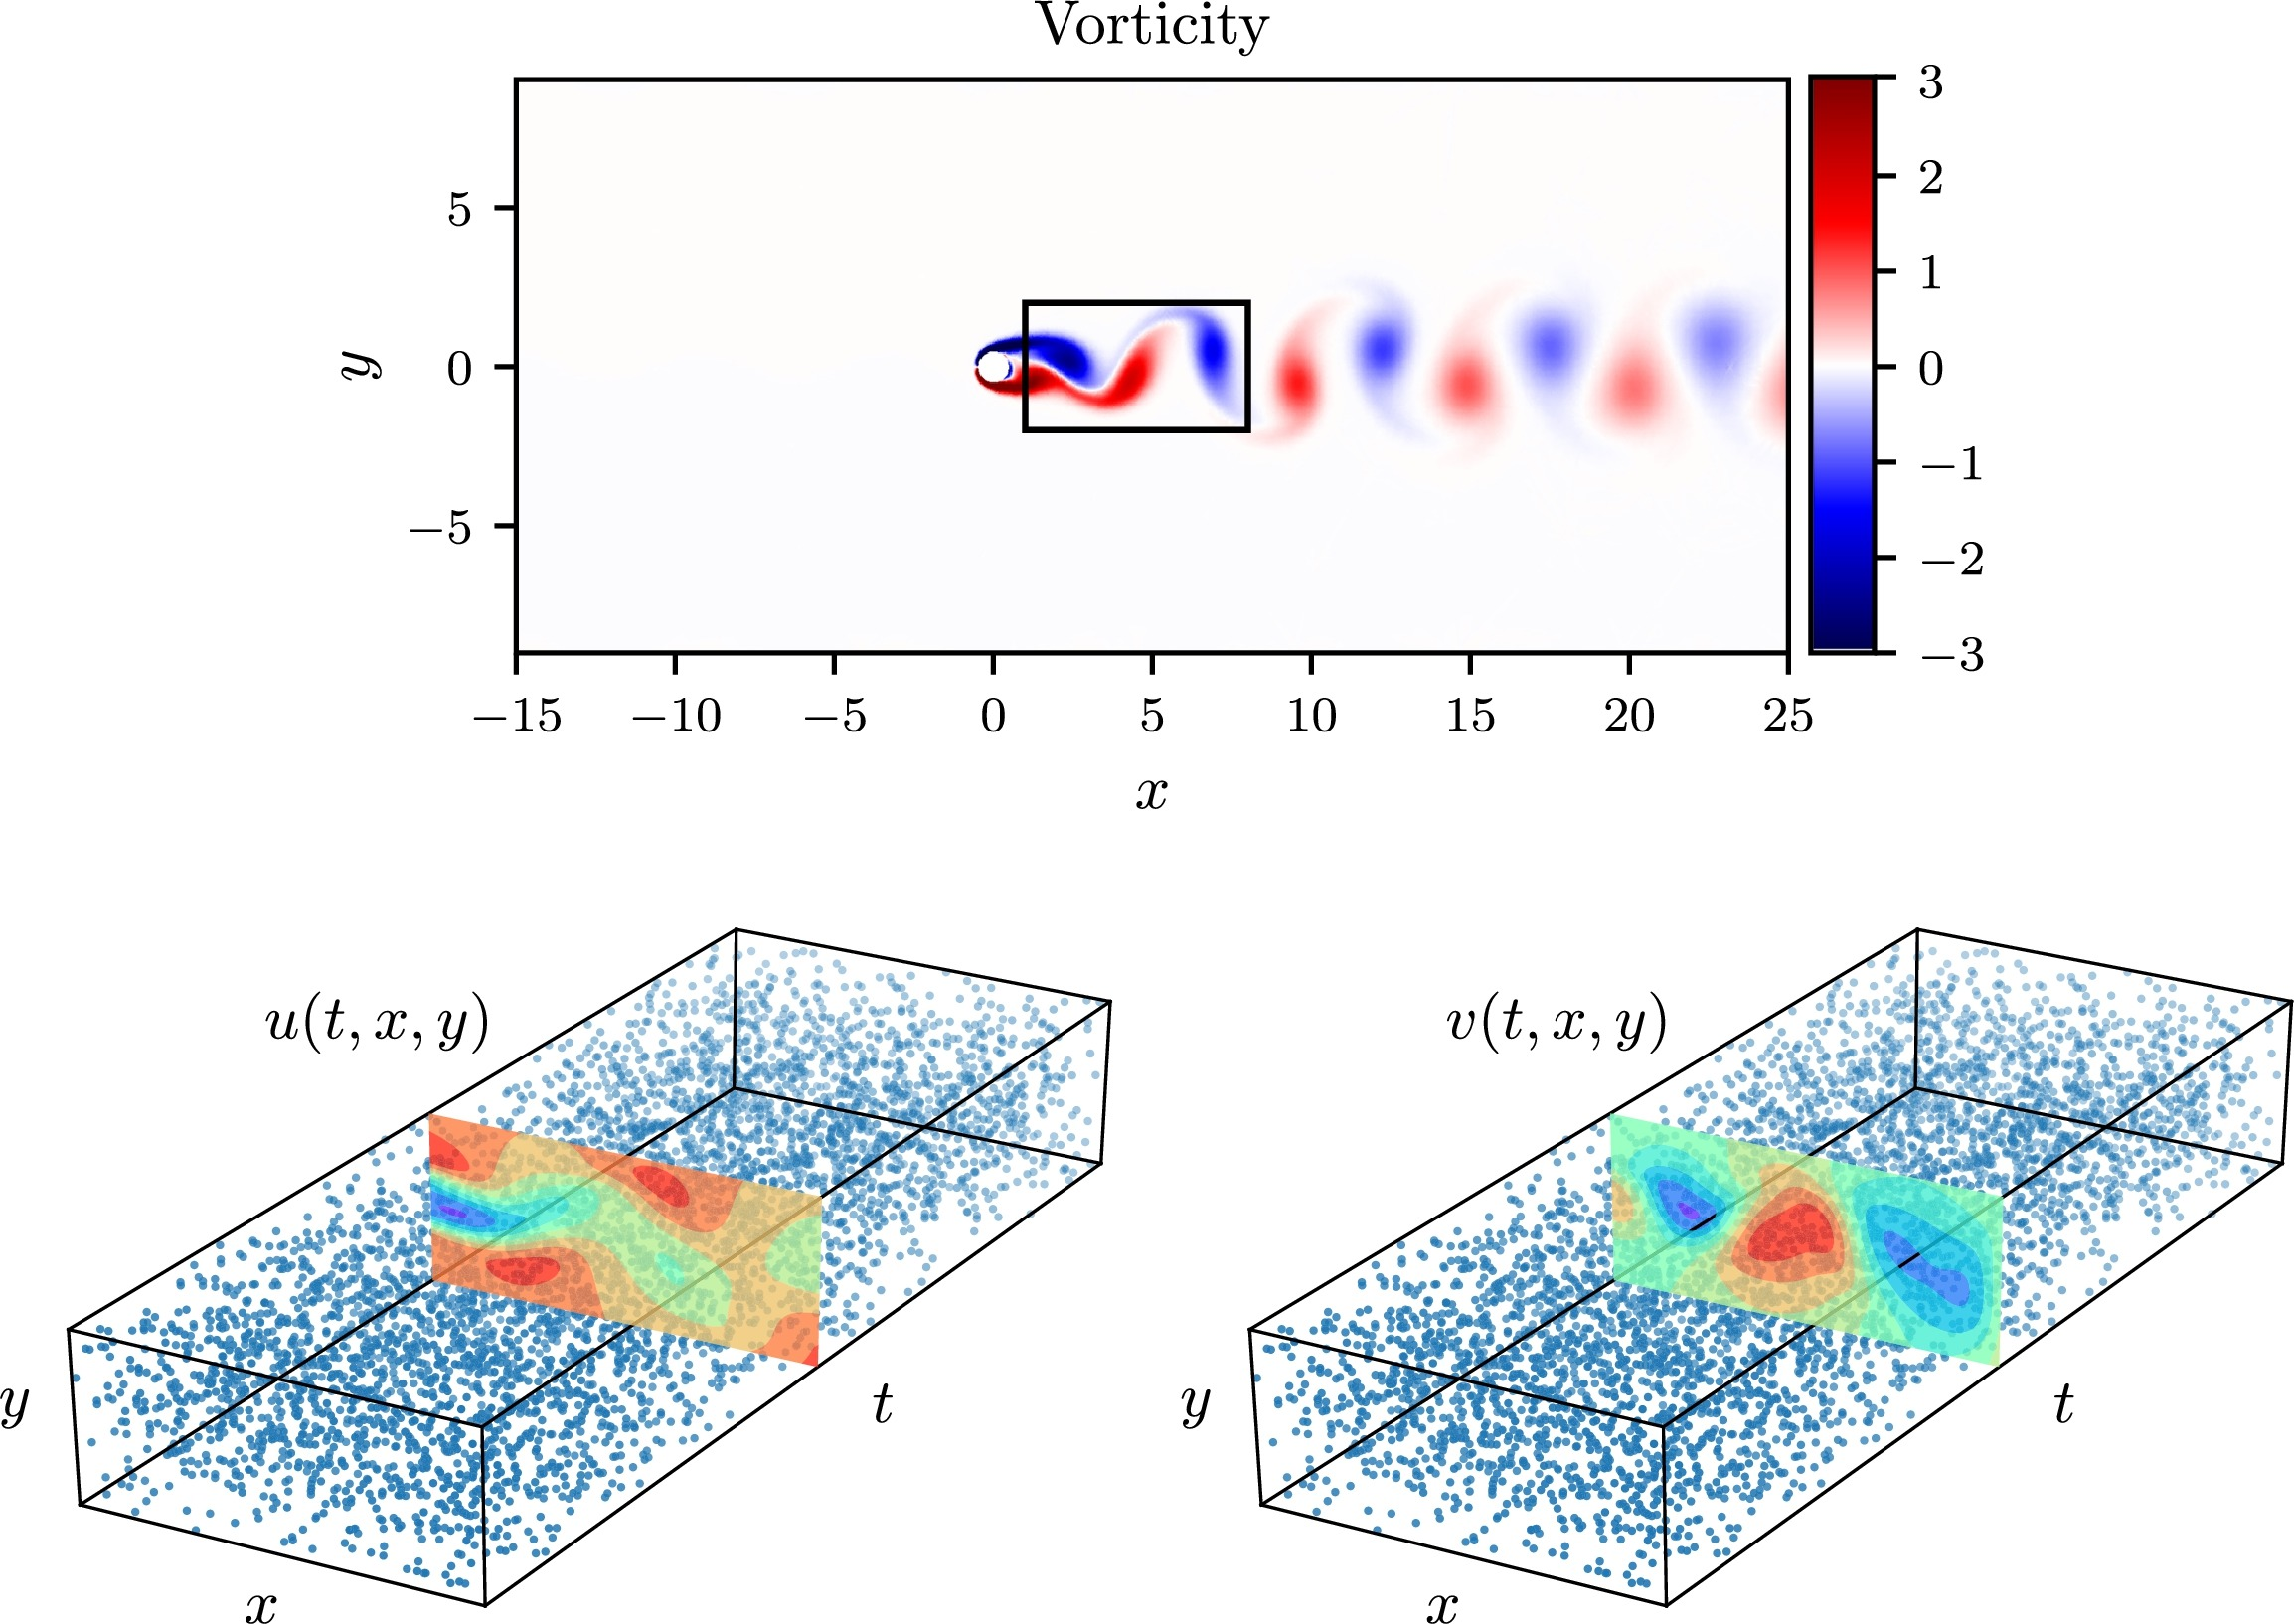
\includegraphics[width=\textwidth]{Figures/PINN Domain.jpg}
    \caption{(Top) Incompressible flow and dynamic vortex shedding past a circular cylinder at Re = 100. Notice the black rectangle outlining the extent of the training/testing data for our PINN. (Bottom) Location of the training data points and the testing data slices in the $u(t,x,y)$ and $v(t,x,y)$ arrays. \cite{Raissi2019}}
    \label{fig:Pinn Domain}
\end{figure}

\subsubsection{PINN Model Setup}
I wrote the PINN model in terms of Python classes. First, I wrote the ``NeuralNetwork'' class that uses abstract methods to enforce essential neural network methods (\texttt{initialize\textunderscore NN}, \texttt{neural\textunderscore net}, \texttt{loss}, \texttt{train}, and \texttt{predict}) on classes that inherit from it. Next I had the class ``PhysicsInformedNN'' inherit from ``NeuralNetwork'', where, in addition to implementing the required methods, I also implemented additional utility methods to help with model initialization and physics-informed equation loss.

\subsubsection{PINN Input-Output Handler}
To handle all the data input, output, and preparation when training and testing the PINN, I implemented the I/O handler class ``NavierStokesPINN\textunderscore IO''. The methods included in this I/O handler class help with data loading and data reduction (\texttt{parse\textunderscore data\textunderscore file}), randomly selecting training data (\texttt{select\textunderscore training\textunderscore data}), selecting data for testing (\texttt{select\textunderscore test\textunderscore data}), and saving model prediction results (\texttt{save\textunderscore predict\textunderscore data}, and \texttt{save\textunderscore multi\textunderscore predict\textunderscore data}). Since several methods in this class depend on the implementation of another class method, I have implemented exception checks to make sure methods in I/O handler are used in a proper order.

\subsubsection{PINN Plotting Handler}
I also implemented a simple plotter class called ``NavierStokesPINN\textunderscore Plotter''that can take the I/O Handler class as an input and use parsed data as well as saved model prediction data to create and save two-dimensional plots comparing model prediction and exact ground truth values for each predicted variable ($u$, $v$, and $p$).

\subsubsection{Example PINN Model Run}
\begin{lstlisting}[language = Python]
import numpy as np
import tensorflow as tf
import matplotlib.pyplot as plt
from navier_stokes_pinn.PINN import PhysicsInformedNN
from navier_stokes_pinn.input_output import NavierStokesPINN_IO
from navier_stokes_pinn.plotting import NavierStokesPINN_Plotter


IO_manager = NavierStokesPINN_IO("navier_stokes_pinn/data", "navier_stokes_pinn/output")
IO_manager.parse_data_file('cylinder_nektar_wake.mat')

# Selecting training data
IO_manager.select_training_data(N_train=5000)

# Extract training data from IO_manager
training_data = IO_manager.training_data

# Casting the training data into tensorflow
x_train = tf.cast(training_data['x_train'], dtype=tf.float32)
y_train = tf.cast(training_data['y_train'], dtype=tf.float32)
t_train = tf.cast(training_data['t_train'], dtype=tf.float32)
u_train = tf.cast(training_data['u_train'], dtype=tf.float32)
v_train = tf.cast(training_data['v_train'], dtype=tf.float32)

# Setting model architechture
layers = [3, 20, 20, 20, 20, 20, 20, 20, 20, 2]

# Setting Reynold's Number
Re = 100

# Initializing the PINN model
# Model training support TensorFlow 2 and GPU acceleration
model = PhysicsInformedNN(x_train, y_train, t_train, u_train, v_train, Re, layers)
# Train PINN model
model.train(2000, learning_rate=1e-3)
# Select test data at a time snapshot to test run inference and test the trained model
time_snapshot = 100
IO_manager.select_test_data(time_snapshot)
test_data = IO_manager.test_data
# Run inference and save predicted data
IO_manager.save_predict_data(model, 'example_prediction_100.npz')

# Plot the predicted data and save the plot with plotting class
Plot_manager = NavierStokesPINN_Plotter("navier_stokes_pinn/data", "navier_stokes_pinn/plots", IO_manager)
# Saves the u, v. and p values at the timestep 100
Plot_manager.plot_compare_predictions('example_prediction_100.npz', time_snapshot)
\end{lstlisting}

\subsection{Unit Testing}









